%qqqqqqqqqqqqqqqqqqqqqqqqqqqqqqqqqqqqqqqqqqqqqqqqqqqqqqqqqqqqqqqqqqqqqqqqq
%Quote
\begin{savequote}[50mm]
‘‘Equipped with his five senses, man explores the universe around him and 
calls the adventure Science’’
\qauthor{Edwin Hubble}
\end{savequote}
%*************************************************************************




%#########################################################################
\chapter{Preliminaries}
\label{cha:Introduction}


%Reviewed
‘‘What is our place in the cosmos?’’ This is one of the simpler and 
trans\-cendental question that human beings have wondered from ancient 
times; furthermore, this, being powered by our innate curiosity, has led to 
a relatively understandable and structured picture of our Universe. Despite 
of that, this knowledge is very new regarding to our whole history, so the 
astronomy can only be considered as a scientific rigorous discipline since 
the seventeenth century.


%#########################################################################





%*************************************************************************
%Prehistory
\section{Prehistory}
\label{sec:Prehistory}


%Reviewed
Almost in every scientific discipline, a significant theoretical development 
is accompanied by a technical and instrumental improvement. That is why at 
the beginning of the seventeenth century, Johannes Kepler could establish 
his three well-known empirical laws of the planetary movements based upon 
the very precise data of astronomical bodies compiled by Tycho Brahe. This 
event was very remarkable in the history of the astronomy since it was the 
first of many strikes against the well established anthropocentric notion 
of the cosmos. Although Kepler's laws constituted the most crucial test to 
the Nicolaus Copernicus's heliocentric model, it was only until 1685, when 
Isaac Newton formulated the law of universal gravitation (from which can be 
derived all the Kepler's laws), when the astronomers could count with 
enough powerful theoretical tools to start a depth and serious discussion 
about the real nature of our universe on scales bigger than the solar 
system, and thus inaugurating the \textit{sciences of gravity} 
\cite{longair2008}.


%Reviewed
After the establishment of the law of universal gravitation, the next 
significant theo\-retical achievement in this area came in the centuries 
eighteenth and nineteenth with the development of classical mechanics, i.e.
Hamiltonian and Lagrangian formalism, and powerful numerical tools. All
those achievements propelled the study of key topics like the many body 
problem, chaotic phenomenons, etc. Allowing a depth understanding of the 
dynamic of complex gravitational systems, such as planetary systems, star 
clusters, etc. 


%Reviewed
Parallel to the previous theoretical advances, on the observational branch 
was beginning to arise the idea of \textit{island universe}, from which 
would evolve the concept of galaxy. All of this was powered by the 
development of the telescope, furthermore allowing to understand that  
galaxies are just a large collection of stars like our sun. It was also 
very remarkable the pioneer work of William Herschel, who tried to build a
complete map of our galaxy determining distances from the assumption of 
stars with the same intrinsic luminosity and with the inverse square law 
for the intensity decay (see figure \ref{fig:HerschelModel}). 
Although his results were very imprecise due to the incorrect assumption 
on which were based, the importance of his work lies on the recognition of 
some structure (disk-like) for our galaxy. 


%.........................................................................
%Herschel Model of Our Galaxy
\begin{figure}[htbp]
	\centering
	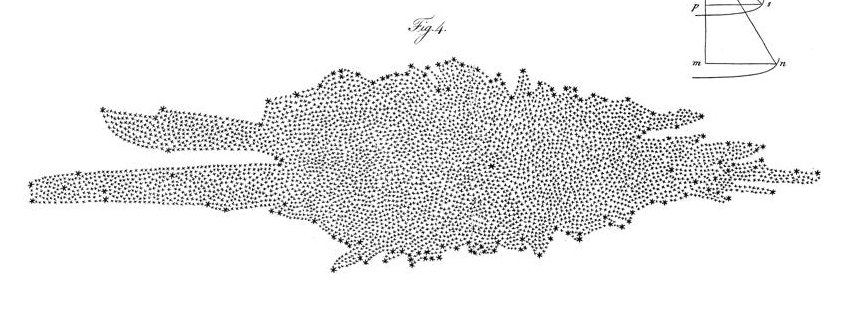
\includegraphics[width=1.0\textwidth]
	{./figures/1_introduction/Herschel_Model.png}
	
	\caption{\small{William Herschel's model for our galaxy based upon a 
	count of stars with the assumption of equal intrinsic luminosity.
	\cite{Herschel1785}.}}
	
	\label{fig:HerschelModel}
\end{figure}
%.........................................................................
\newpage

%Reviewed
Another important observational question, that was emerging among 
scientists by that time, was the existence of \textit{island universes} 
like ours. It was already well-known the existence of extended objects 
that do not fit to the definition of stars or planets, like nebulae, 
planetary disks and galaxies. Even, William Herschel and his son, John 
Herschel, contributed with the realization of a large (for the epoch) 
catalogue of extended bodies known as \textit{Catalogue of Nebulae and 
Clusters of Stars} and a subsequent improved and expanded version finished 
by John Dreyer in 1888, \textit{New General Catalogue of Nebulae and 
Clusters of Stars}, which together with \textit{Index Catalogues} of 1895 
and 1908 constitute a large collection of bodies widely used in current 
astronomy, referred with the abbreviations \textit{NGC} and \textit{IC} 
respectively \cite{longair2008}. Despite of those observational advances, 
the real nature of these objects was a complete mystery, especially if they 
lie within our own galaxy or are completely independent systems. 


%Reviewed
This question remained unsolved until the twentieth century, and together 
with the indetermination of the real size of the universe, were the two 
big issues treated on the well-known \textit{Great Debate}, or also called 
the \textit{Shapley-Curtis Debate}. In this important event in the history 
of astronomy, the astronomers Harlow Shapley and Herber Curtis discussed 
about these topics, giving, respectively, different arguments for and 
against if these objects are within our galaxy and if the Milky Way is our 
whole universe or not \cite{Curtis1921} \cite{Shapley1921}. Despite of 
that, their arguments were not very conclusive and the definitive solution 
to these issues had to wait until 1924, when Edwin Hubble measured the 
distance to Andromeda Galaxy (M31 or NGC 224) and demonstrated 
unquestionably the real extragalactic nature of this object, and in 
following years for other ones \cite{Hubble1926}. This achievement along 
with the observational verification of the expanding universe (also due to 
Hubble) were the beginning of the modern observational cosmology.


%Reviewed
It also happened in the twentieth century a key event for the modern 
sciences of gravity, Albert Einstein formulated his theory of General 
Relativity \cite{Einstein1916}, challenging and changing completely the 
previous conception of space and time and laying the foundation of current 
cosmology picture.



%*************************************************************************




%*************************************************************************
%The current cosmology picture
\section{The Current Cosmology Picture }
\label{sec:TheCurrentCosmologyPicture}


%Reviewed
The theoretical basis on which are based the theory of general relativity
began to arise with the zenith of non-euclidean geometries in the 
nineteenth century and the beginning of twentieth, when it was demonstrated 
that the Euclid's fifth postulate is not needed to build self-consistent 
geometries, thus giving rise to non-planar geometries (see figure 
\ref{fig:NonEuclidean}). In particular, it was highlighted the work of 
Nikolai Lobachevsky, father of non-euclidean geometries, and Bernhard 
Riemman, the founder of the Riemannian geometry.


%.........................................................................
%Herschel Model of Our Galaxy
\begin{figure}[htbp]
	\centering
	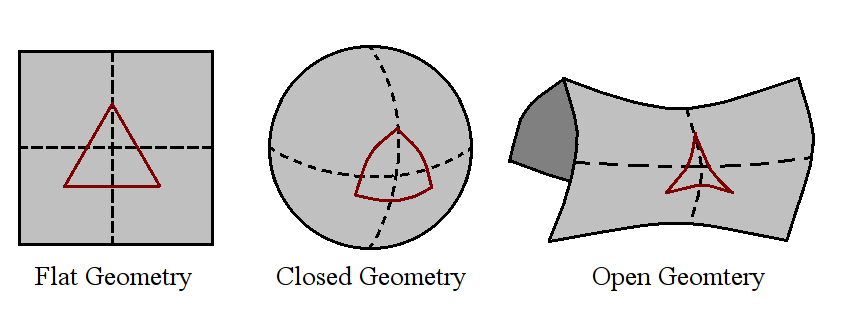
\includegraphics[width=0.9\textwidth]
	{./figures/1_introduction/Non_Euclidean.png}
	
	\caption{\small{Different geometries according to variations on	
	Euclid's fifth postulate.}}
	
	\label{fig:NonEuclidean}
\end{figure}
%.........................................................................


%Reviewed
In spite of these first developments contributed widely to the current 
cosmological paradigm, bringing forward discussions on what kind of 
geometry the universe has, the concepts of space and time were completely 
misunderstood yet, being interpreted as unrelated and absolute entities.
That is why the foundation of the theory of general relativity opened the
door to our whole current understanding.


%Reviewed
Once obtained the equations of metric field of the general relativity, it 
was possible to build global and self-consistent models of the universe.
A first rough attempt was also due to Einstein, who formulated, influenced
by his own belief, a static and closed model of the universe. To achieve it,
he must use the well-known cosmological constant in order to compensate the
expansion/contraction obtained naturally by the theory.


%Reviewed
Few year later, Aleksander Friedmann demonstrated on two articles a 
set of solutions for closed and hyperbolic universes'\ expanding from a
singularity \cite{FriedmanA} \cite{FriedmanB}. These expanding solutions 
were in agreement with the observations made by Hubble for redshift of 
far galaxies. Because of that, the inclusion of the cosmological constant 
for stationary solutions it is historically known and recognized by 
Einstein himself as the biggest blunder of his life. This theoretical 
finding prompted a set of studies on the real nature of the universe in 
the light of those new solutions, like large-scale dynamics, global 
geometry and precise measurements of different cosmological parameters of
those models.


%Reviewed
The next important advance came with the formulation of the Big Bang 
theory by George Gamow. This theory proposes that early stages of 
the universe had been very dense and hot, starting from a singularity and 
reaching the current stage, a constantly cooling and expanding universe. 
All this is in agreement with the Friedmann's solutions. One of the first 
predictions of this theory was the early nucleosynthesis, which is 
responsible of the creation of heavy elements like helium and lithium 
through fusion reactions of primordial hydrogen. Because of the current 
abundances of helium and lithium cannot be given account by the standard
nuclear processes in stars, this was the first of many achievement of the 
Big Bang theory; furthermore the early nucleosynthesis was later 
demonstrated by Ralph Alpher and Robert Herman and it has been 
observationally corroborated very precisely nowadays.

\
%.........................................................................
%Cosmic Background Radiation
\begin{figure}[htbp]
	\centering
	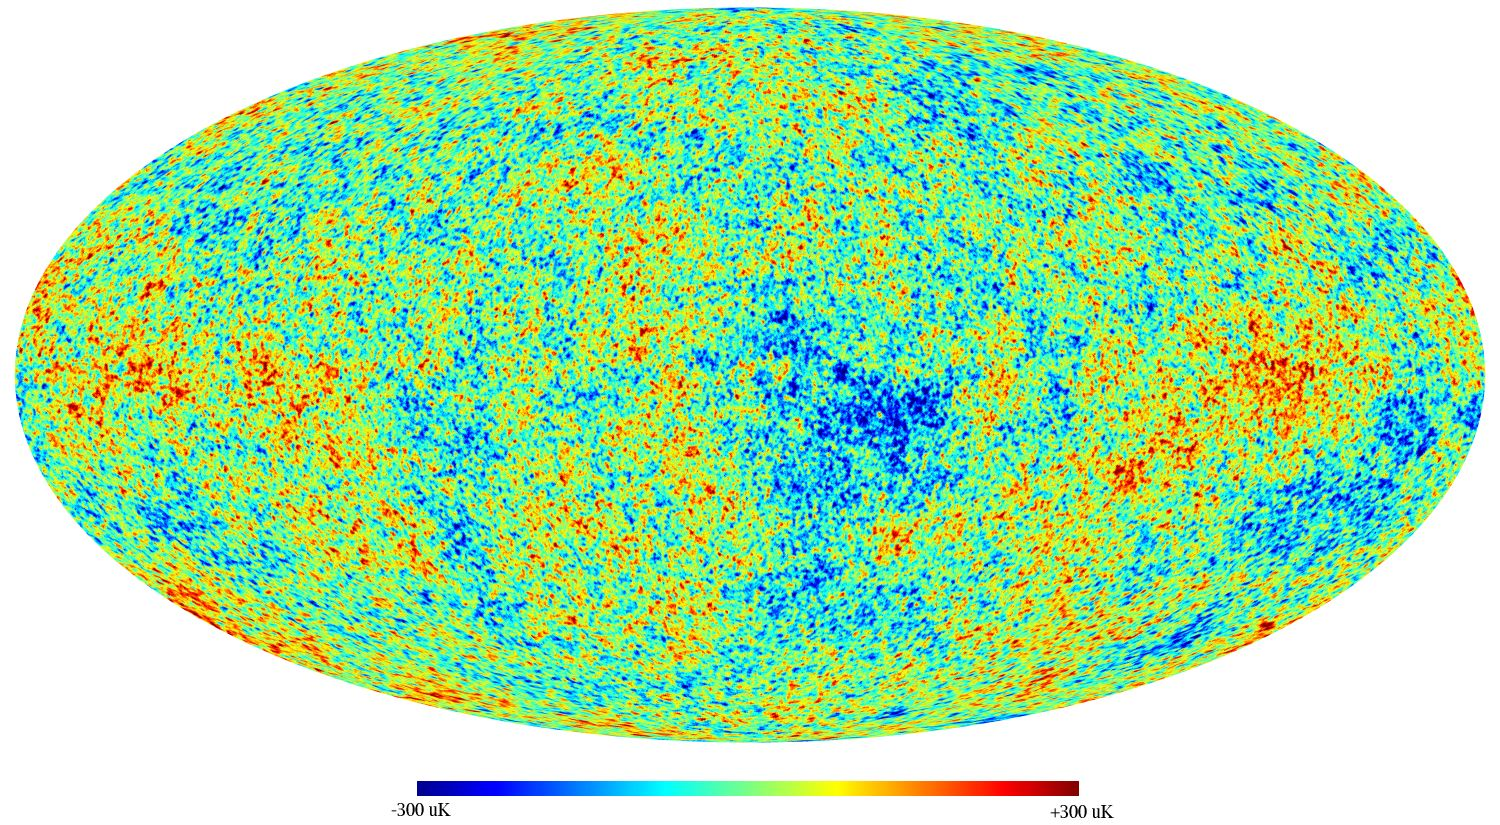
\includegraphics[width=0.8\textwidth]
	{./figures/1_introduction/CMB.png}
	
	\caption{\small{Cosmic background radiation. Taken from 
	\url{http://upload.wikimedia.org/wikipedia/commons/3/3c/Ilc_9yr_moll4096.png}}}
	
	\label{fig:CMB}
\end{figure}
%.........................................................................


%Reviewed
The next remarkable prediction of the Big Bang theory was the current 
existence of a residual black-body radiation from early stages, when,
due to the conditions of high density and temperature, the universe was 
radiation-dominated. This remainder was verified observationally by Arno 
Penzias and Robert Wilson in 1965 with the discovery of the cosmic 
background radiation (CMBR). The spectrum of this residual radiation proved 
to be produced by an almost perfect black-body with a characteristic 
temperature of  $T = 2.725$ K. These predictions have made this theory 
being adopted as a fundamental part of the standard cosmological paradigm.


%Reviewed
Although the discovery of the CMBR was certainly one the most important 
hits of the astronomy along the century twenty, as it has been established 
in many scientific disciplines, new answers lead to new questions. In this 
case, the horizon problem. This is originated by the high angular isotropy 
measured from the CMBR spatial spectrum (see figure \ref{fig:CMB}), which 
suggests a causal connection between regions of the universe very far apart 
from each other that, in theory, they should not be correlated. The widely 
accepted solution to this problem was proposed by Alan Guth in 1980, the 
inflationary theory. This postulates an exponential expansion of the early 
universe powered by a scalar field, the inflaton. During the time of 
expansion, vacuum quantum fluctuations of each field present in the 
universe was magnified by the expansion itself, producing small 
perturbations in the density field, from which would evolve current 
large-scale structures. According to this, the inflationary theory can 
explain satisfactorily the problem of small perturbations of the very 
early universe, becoming thus an essential part of the current paradigm. 


%Reviewed
The existence of dark matter was proposed since early 1930s, initially by
Jan Oort in 1932 and then by Fritz Zwicky in 1933, in order to give account
of non-luminous matter of galaxies and galaxy clusters, which is manifested
through dynamical interactions of their single components, like stars or 
galaxies in the case of clusters. In spite of that, the real nature of this 
new type of matter remained as a complete mystery. In 1984 Joel Primack, 
George Blumenthal, Sandra Moore and Martin Rees proposed a model called 
cold dark matter (CDM), in which is postulated that dark matter is made of 
certain unknown type of non-relativistic particle which only interacts 
gravitationally and electromagnetically (more weakly). Under this scheme, 
it is possible to demonstrate that large-scale structure formation follows 
a \textit{top-down} hierarchical process, in which the smallest structures 
are formed first and the biggest, composed by the first, are formed later. 
This has been observationally verified through galaxy surveys (see section
\ref{sec:CosmologicalObservations}).


%Reviewed
In the 1990s, some cosmological observations suggested an accelerated rate
of expansion of the universe, which only can be explained (see subsection 
\ref{subsec:SimpleSolutionsOfTheUniverse}) with the inclusion of the 
cosmological constant in the field equations of the general relativity.
Because this constant can be placed as an energy density term with negative
pressure, the term of \textit{dark energy} was quickly coined, even though 
its real nature is completely unknown. Very precise measurements have 
proved that our universe is currently vacuum-dominated, reaching $70 \%$
of all content of matter-energy of it. This last fact completes our overall
picture of the current cosmological paradigm and it is called standard 
$\Lambda$CDM model or concordance model.


\
%.........................................................................
%Local Group
\begin{figure}[htbp]
	\centering
	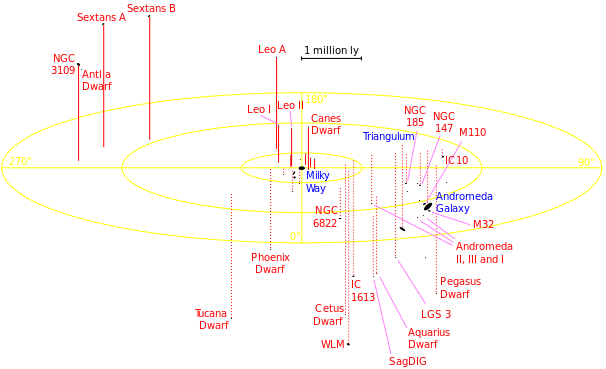
\includegraphics[width=1.0\textwidth]
	{./figures/1_introduction/LocalGroup.png}
	
	\caption{\small{Local Group. Taken from 
	\url{http://commons.wikimedia.org/wiki/File:Local_Group.svg}}}
	
	\label{fig:LocalGroup}
\end{figure}
%.........................................................................


%Reviewed
The local group (LG) is a local system composed of 30 galaxies approximately, 
which interact gravitationally between them and evolve relatively isolated 
from other large-scale structures. The Milky Way and Andrómeda (M31) 
galaxies are its more representative members and even in this work we shall 
simplify the local group just as systems of two galaxies similar to these 
(see figure \ref{fig:LocalGroup}).


%Reviewed
The importance of our local group in a cosmological context is because it
is by far the best known large-scale structure, thereby allowing to verify
some current predictions of the concordance model. Among the issues 
originated by these predictions, we highlight the over abundance of 
satellite galaxies in the Milky Way, the possible link between the flows
of the Magellanic clouds and M31 galaxy, tidal forces in the local group,
the kinematic of M31 and Milky Way galaxies in a cosmological context 
\cite{forero2013} and the influence of the cosmological environment on the
formation properties of systems like the local group.



%*************************************************************************





%*************************************************************************
%Cosmological observations
\section{Cosmological Observations}
\label{sec:CosmologicalObservations}
	
	
%Reviewed
The boom produced by the space age along with the significant 
technological development of measuring instruments and sensors have 
powered enormously observational research in cosmology, thereby allowing, 
together with the theoretical advances previously discussed, to reach the 
current cosmological picture. Next, we shall present some of the larger
and more important observational projects in cosmology and which are 
widely used in current research.



	%---------------------------------------------------------------------
	%2DF Galaxy Redshift Survey
	\subsection*{2DF Galaxy Redshift Survey}
	\label{subsec:2DFGRS}
	%---------------------------------------------------------------------
	
	
%Reviewed
The 2DF Galaxy Redshift Survey (2DFGRS), or Two-Degree-Field Galaxy 
Redshift Survey\footnote{Official web page of the project at 
\url{http://magnum.anu.edu.au/~TDFgg/}.}, is a galaxy redshift survey 
performed within an angular area of $1500$ square degrees of regions near 
to the north and south galatic poles in order to avoid extinction produced 
by the galactic disk. This survey was made by the $3.9$ m telescope of the 
Anglo-Australian observatory from 1997 to 2002. Among the main results of 
this survey are remarkable the mapping of the local structure of the 
large-scale environment around the local group of galaxies. This was 
achieved through photometric measurements of $382\ 323$ objects within a 
redshift range of $z=0.3$ to $z=0.0$. It is also remarkable the measuring 
of the density parameter of non-relativistic matter (dark + baryonic) of
the standard cosmological model.
	

	
	%---------------------------------------------------------------------
	%Sloan Digital Sky Survey
	\subsection*{Sloan Digital Sky Survey}
	\label{subsec:SDSS}
	%---------------------------------------------------------------------


%Reviewed
The Sloan Digital Sky Survey (SDSS), like the 2DFGRS, is a redshift survey 
of the large-scale universe made by the $2.5$ m telescope of the Apache 
Point observatory in New Mexico since 2000.



%.........................................................................
%SDSS
\begin{figure}[htbp]
	\centering
	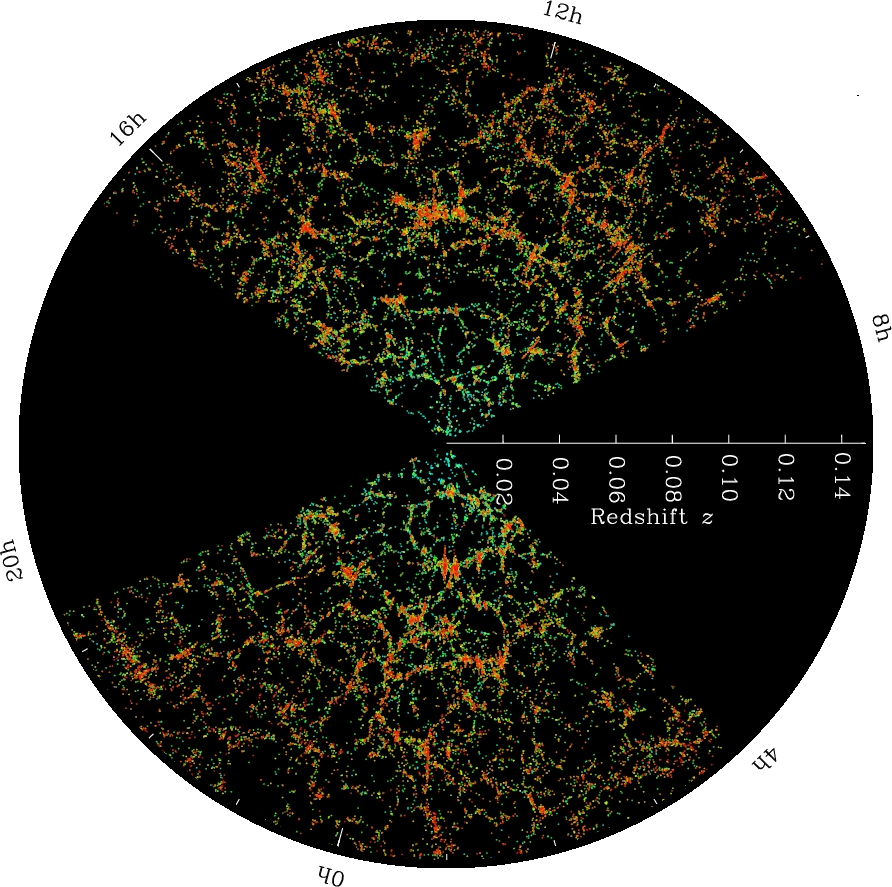
\includegraphics[width=0.6\textwidth]
	{./figures/1_introduction/SDSS.png}
	
	\caption{\small{Map of the large-scale universe according to the Sloan 
	Digital Sky Survey. Taken from the official web page of the project 
	\url{http://www.sdss.org/}}}
	
	\label{fig:SDSS}
\end{figure}
%.........................................................................


%Reviewed
The survey covers an area significantly larger than 2DFGRS, 
approximately $7500$ square degrees, and has catalogued around $2$ million
of objects, thereby allowing to build a map of the large-scale universe in 
which it was first seen the structure of the cosmic web (see figure 
\ref{fig:SDSS}).


	
	%---------------------------------------------------------------------
	%WMAP
	\subsection*{WMAP}
	\label{subsec:WMAP}
	%---------------------------------------------------------------------


%Reviewed
The Wilkinson Microwave Anisotropy Probe (WMAP), is a NASA spacecraft 
launched in 2001 and placed in the lagrange point L2. Its main objective
is to measure, with very high precision, small temperature contrasts and 
polarization of the cosmic background radiation (see figure \ref{fig:CMB}).
Approximately every two years, NASA releases the accumulated results 
obtained, called as WMAP1, WMAP3, WMAP5, WMAP7 and finally WMAP9 for data 
released in 2012. These results have been up to date the most reliable 
proof of the standard cosmological $\Lambda$CDM model. Especially it is
remarkable the precise measuring of the age of the universe, the 
cosmological density parameters, the Hubble's constant, also the 
determination of the global geometry of the universe (flat geometry) and
the confirmation of the inflationary model.


\
%.........................................................................
%Cosmological Parameter of WMAP7
\begin{table}[htbp]
\begin{small}
\centering
\begin{tabular}{|c|c|c|c|} \hline
\cellc{\textbf{Parameter}}		&
\cellc{\textbf{Notation}}		&  
\cellc{\textbf{Value}}			& 
\cellc{\textbf{Unit}}					\\ \hline


Age of universe 			&	$t_0$			&	$13.75 \pm 0.13$	&	Ga 			\\ \hline

Hubble's constant			&	$H_0$			&	$71.0 \pm 2.5$		&   km/(Mpc s)	\\ \hline

Hubble's parameter			&	$h$				&	$0.71 \pm 0.025$	&   --			\\ \hline

Barion density		&	$\Omega_b$		&	$0.0449\pm 0.0027$	&	--			\\ \hline

Dark matter & & & \\
density				&	$\Omega_c$		&	$0.222 \pm 0.026$	&	--			\\ \hline

Dark energy & & & \\
density				&	$\Omega_\Lambda$&	$0.734 \pm 0.029$	&	--			\\ \hline

Radiation & & & \\
density					&	$\Omega_r$		&$8.24 \times 10^{-5}$	&	--			\\ \hline

Amplitude of & & & \\
Fluctuations at $8h^{-1}$ Mpc&	$\sigma^2_8$	&	$0.801 \pm 0.030$	&	--			\\ \hline

Spectral index			&	$n_s$			&	$0.963 \pm 0.014$	&	--			\\ \hline
Reionization & & & \\
optic depth 			&	$\tau$			&	$0.088 \pm 0.015$	&	--			\\ \hline
				
Total density of & & & \\
the Universe	&	$\Omega_0$		&	$1.080\ \mbox{\scriptsize{$+0.093$}}/ 
										\mbox{\scriptsize{$-0.071$}} $&	--				\\ \hline
\end{tabular}
\caption{WMAP7 cosmological parameters \cite{WMAP7}.}
\label{tab:CosmologicalParameters}
\end{small}
\end{table}
%.........................................................................


%Reviewed
In the table \ref{tab:CosmologicalParameters} is tabulated all the results
of the WMAP7 release \cite{WMAP7}, which are widely used in next chapters 
and especially in the different cosmological simulations presented below in
the chapters \ref{cha:N-BodySimulations} and \ref{cha:Results}.



%*************************************************************************